\documentclass{standalone}
\usepackage{unicode-math}
\usepackage{siunitx}
\usepackage{tikz}
\usetikzlibrary{shapes, shapes.geometric}
\usetikzlibrary{graphs, matrix, quotes}

\begin{document}
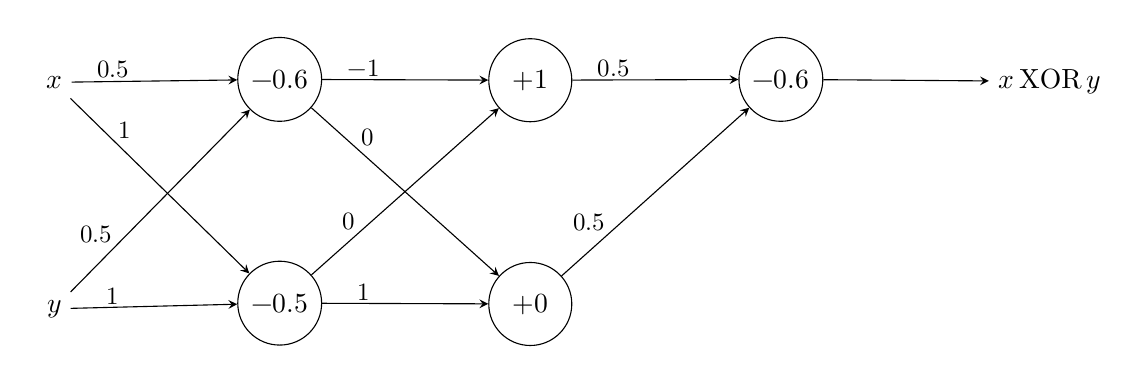
\begin{tikzpicture}[
	neuron/.style={
		draw,
		circle,
		minimum width=3em,
	},
	net/.style={
		matrix of nodes,
		column sep=6em,
		row sep=5em,
		nodes in empty cells,
	},
	>=stealth,
]

\matrix[net] (mat){
	\(x\) & |[neuron]| {\(-0.6\)} & |[neuron]| {\(+1\)} & |[neuron]| {\num{-0.6}}& \(x \operatorname{XOR} y\)\\
	\(y\) & |[neuron]| {\(-0.5\)} & |[neuron]| {\(+0\)}\\
};

% TODO: label the outputs with like "x AND y" for the output of mat-2-2
\graph[
	use existing nodes,
	edge quotes={near start, auto, inner sep=0.1em, font=\small},
] {
	(mat-1-1) ->["\num{0.5}"] (mat-1-2);
	(mat-1-1) ->["\num{1}"] (mat-2-2);
	(mat-2-1) ->["\num{0.5}"] (mat-1-2);
	(mat-2-1) ->["\num{1}"] (mat-2-2);

	(mat-1-2) ->["\num{-1}"] (mat-1-3);
	(mat-1-2) ->["\num{0}"] (mat-2-3);
	(mat-2-2) ->["\num{0}"] (mat-1-3);
	(mat-2-2) ->["\num{1}"] (mat-2-3);
	
	(mat-1-3) ->["\num{0.5}"] (mat-1-4);
	(mat-2-3) ->["\num{0.5}"] (mat-1-4);
	
	(mat-1-4) -> (mat-1-5);
};
\end{tikzpicture}
\end{document}